% DO LE DUY
% 1026-32-2038
% August 04 2020

\documentclass[11pt]{article}
\usepackage[T1]{fontenc}
\usepackage[bitstream-charter]{mathdesign}
\usepackage{amsmath, amsthm} 
\usepackage{geometry}
\usepackage{hyperref}
\usepackage{parskip}
\usepackage{graphicx}
\graphicspath{ {./graphic/} }
\pagenumbering{gobble}
\geometry{left=2cm,right=2cm,top=1cm,bottom=2cm,includeheadfoot}

\title{Practice of Basic Informatics — Final Report \vspace{-2ex}}
\author{by Do Le Duy}

\begin{document}
\maketitle

\section{Introduction}
Our main task is to write a program (or programs) able to obtain the number of terms required to calculate $e$ up to the third decimal position (i.e., $2.718$ ) using both expressions, and plot their convergence from 1 to 100 steps:\\
Napier's constant in expression of series:
\[
e=1+\sum_{n=1}^{\infty}\left(\frac{1}{n !}\right)
\]
Napier's constant in expression of its definition: 
\[
e=\lim _{n \rightarrow \infty}\left(1+\frac{1}{n}\right)^{n}
\]
Our first FORTRAN program will compare the value of the two computation results to $e$ rounded to its third decimal digit and return the number of steps required for the results to reach that value.\\
Our second and third FORTRAN programs will write the parameter of each step from step 1 to 100, their output will be redirected to a data file. Then we will investigate the convergence of the two computations by plotting the values using gnuplot.  

\section[title]{History of Napier’s constant \footnote{$e$ (mathematical constant). (n.d.). In Wikipedia. Retrieved August 01, 2020, from \url{https://en.wikipedia.org/wiki/E_(mathematical_constant)}}}

The Napier’s constant $e$, also known as Euler's number, is a mathematical constant approximately equal to 2.71828 which can be characterized in many ways. The discovery of the constant itself is credited to Jacob Bernoulli in 1683, who attempted to find the value of the following expression in his study of compound interest:
\[ 
\left( 1+ \frac{1}{n} \right)^{n}
\]
The definition of $e$ is the limit of the expression as $n$ approaches infinity. It is also derived to be the base of the natural logarithm, and can also be calculated as the sum of the infinite series:
\[
e=\sum_{n=0}^{\infty} \frac{1}{n !}=\frac{1}{1}+\frac{1}{1}+\frac{1}{1 \cdot 2}+\frac{1}{1 \cdot 2 \cdot 3}+\cdots.
\]
In fact, Euler used this to calculate $e$ up to its 18th decimal. 

The first references to the constant were published in 1618 in the table of an appendix of a work on logarithms by John Napier. However, this did not contain the constant itself, but simply a list of logarithms calculated from the constant. It is assumed that the table was written by William Oughtred. Jacob Bernoulli is credited to discover the constant in 1683 during his study of compound interest. The first known use of the constant, represented by the letter $b$, was in correspondence from Gottfried Leibniz to Christiaan Huygens in 1690 and 1691. Leonhard Euler introduced the letter $e$ as the base for natural logarithms, writing in a letter to Christian Goldbach on 25 November 1731. Euler started to use the letter $e$ for the constant in 1727 or 1728, in an unpublished paper on explosive forces in cannons, and the first appearance of $e$ in a publication was in Euler's Mechanica (1736). While in the subsequent years some researchers used the letter $c$, the letter $e$ was more common and eventually became standard.

\section{Fortran Programs}
\subsection{First Program}
Following is the first Fortran Program used to obtain the number of steps required to calculate $e$ up to its third decimal position. The output of the program is shown in the next section. 
\begin{verbatim}
PROGRAM  Exponential_3th_decimal
   IMPLICIT  NONE
! Initialize some variables  
   INTEGER         :: n         
   DOUBLE PRECISION:: one_over_n    
   DOUBLE PRECISION:: Term
   DOUBLE PRECISION:: Sum      
   REAL            :: e_third_decimal
   
   e_third_decimal = ANINT(EXP(1.0)*1000)/1000.0
   
! First Expression
   n = 0                                ! # of terms used starts with 0
   Term  = 1.0                          ! initialize the term as 1
   Sum   = 1.0                          ! initialize the sum as 1

   DO                                   ! for each term, compute
      n = n + 1                         ! indicate of current term
      one_over_n = 1.0 / n
      Term  = Term * one_over_n         ! value of current term
      Sum   = Sum + Term                ! add new term to sum
      IF (Sum > e_third_decimal)  EXIT  ! if pass e with third decimal, exit
   END DO

   WRITE(*,*)  'After', n, 'steps:'
   WRITE(*,*)  'e             = ', Sum
   WRITE(*,*)  'Abs(Error)    = ', ABS(Sum - EXP(1.0))
   
   
 ! Second Expression
   n = 0                               ! # of terms used starts with 0
   Term  = 1.0                         ! initialize the term as 1
 
   DO                                  ! for each term, compute
      n = n + 1                        ! n indicate of current term
      one_over_n = 1.0 / n
      Term  = (1 + one_over_n)**n      ! value of current term
      IF (Term > e_third_decimal)  EXIT! if pass e with third decimal, exit
   END DO
   
   WRITE(*,*)  'After', n, 'steps:'
   WRITE(*,*)  'e             = ', Term
   WRITE(*,*)  'Abs(Error)    = ', ABS(Term - EXP(1.0))

END PROGRAM  Exponential_3th_decimal
\end{verbatim}
\subsection{Second and Third Program}
\begin{itemize}
\item  The second program is for investigating the convergence of the expression: 
\[
e=1+\sum_{n=1}^{\infty}\left(\frac{1}{n !}\right).
\]
\begin{verbatim}
PROGRAM  Exponential_first_expression
   IMPLICIT  NONE
! Initialize some variables  
   INTEGER         :: n         
   DOUBLE PRECISION:: one_over_n    
   DOUBLE PRECISION:: term
   DOUBLE PRECISION:: sum_terms      

! First Expression
   n = 0                                ! # of terms used starts with 0
   term  = 1.0                          ! initialize the term as 1
   sum_terms   = 1.0                    ! initialize the sum as 1

   DO                                   ! for each term, compute
      n = n + 1                         ! indicate of current term
      one_over_n = 1.0 / n
      term  = term * one_over_n         ! value of current term
      sum_terms   = sum_terms + term    ! add new term to sum
      WRITE(*,*)  n, sum_terms
      IF (n == 100)  EXIT               ! if n reaches 100, exit
   END DO

END PROGRAM  Exponential_first_expression
\end{verbatim}

\item The third program is for investigating the convergence of the expression: 
\[
e=\lim _{n \rightarrow \infty}\left(1+\frac{1}{n}\right)^{n}.
\]
\begin{verbatim}
PROGRAM  Exponential_second_expression
   IMPLICIT  NONE
! Initialize some variables  
   INTEGER         :: n         
   DOUBLE PRECISION:: one_over_n    
   DOUBLE PRECISION:: term

 ! Second Expression
   n = 0                               ! # of terms used starts with 0
   term  = 1.0                         ! initialize the term as 1
 
   DO                                  ! for each term, compute
      n = n + 1                        ! n indicate of current term
      one_over_n = 1.0 / n
      term  = (1 + one_over_n)**n      ! value of current term
      WRITE(*,*)  n, term
      IF (n == 100)  EXIT              ! if n reaches 100, exit
   END DO

END PROGRAM  Exponential_second_expression
\end{verbatim}
\end{itemize}
\section{Response by the computer}
Following is the output of the first program. 
\begin{verbatim}
   After           6 steps:
   e             =    2.7180555622403819     
   Abs(Error)    =    2.2618367026261410E-004
   After        4821 steps:
   e             =    2.7180000473061505     
   Abs(Error)    =    2.8169860449400730E-004   
\end{verbatim}

The output of the second and third program are redirected into data files data1.dat and data2.dat respectively, which will be uploaded to Panda. 
\newpage
\section{gnuplot Instructions}
The instructions to plot the two data files is written in the data1.plt and data2.plt respectively. The content of the two files is as below:
\begin{itemize}
   \item data1.plt file
\begin{verbatim}
# plot file data1.plt

set xlabel 'Number of steps'
set ylabel 'Results of Computation'
set yrange [1.8:3]
set xrange [0:100]
set terminal wxt size 2048, 1536 font ",16"
set style line 1 \
    linecolor rgb '#0060ad' \
    linetype 1 linewidth 2 \
    pointtype 7 pointsize 1.5

plot 'data1.dat' title "Series Expression" with linespoints linestyle 1
\end{verbatim}
\item data2.plt file
\begin{verbatim}
# plot file data2.plt

set xlabel 'Number of steps'
set ylabel 'Results of Computation'
set yrange [1.8:3]
set xrange [0:100]
set terminal wxt size 2048, 1536 font ",16"
set style line 1 \
    linecolor rgb '#8B0000' \
    linetype 1 linewidth 2 \
    pointtype 7 pointsize 1.5

plot 'data2.dat' title "Limit Definition Expression" with linespoints linestyle 1
\end{verbatim}
\end{itemize}
These two files will also be uploaded on Panda. 
\newpage
\section{Results and Discussion}
The first expression only requires 6 terms in order to calculate $e$ with precision of three decimals. But the second expression requires up to 4821 terms to accomplish the same. 

The plots that demonstrated the convergence of each expression are as below:
\begin{figure}[h]
   \centering
   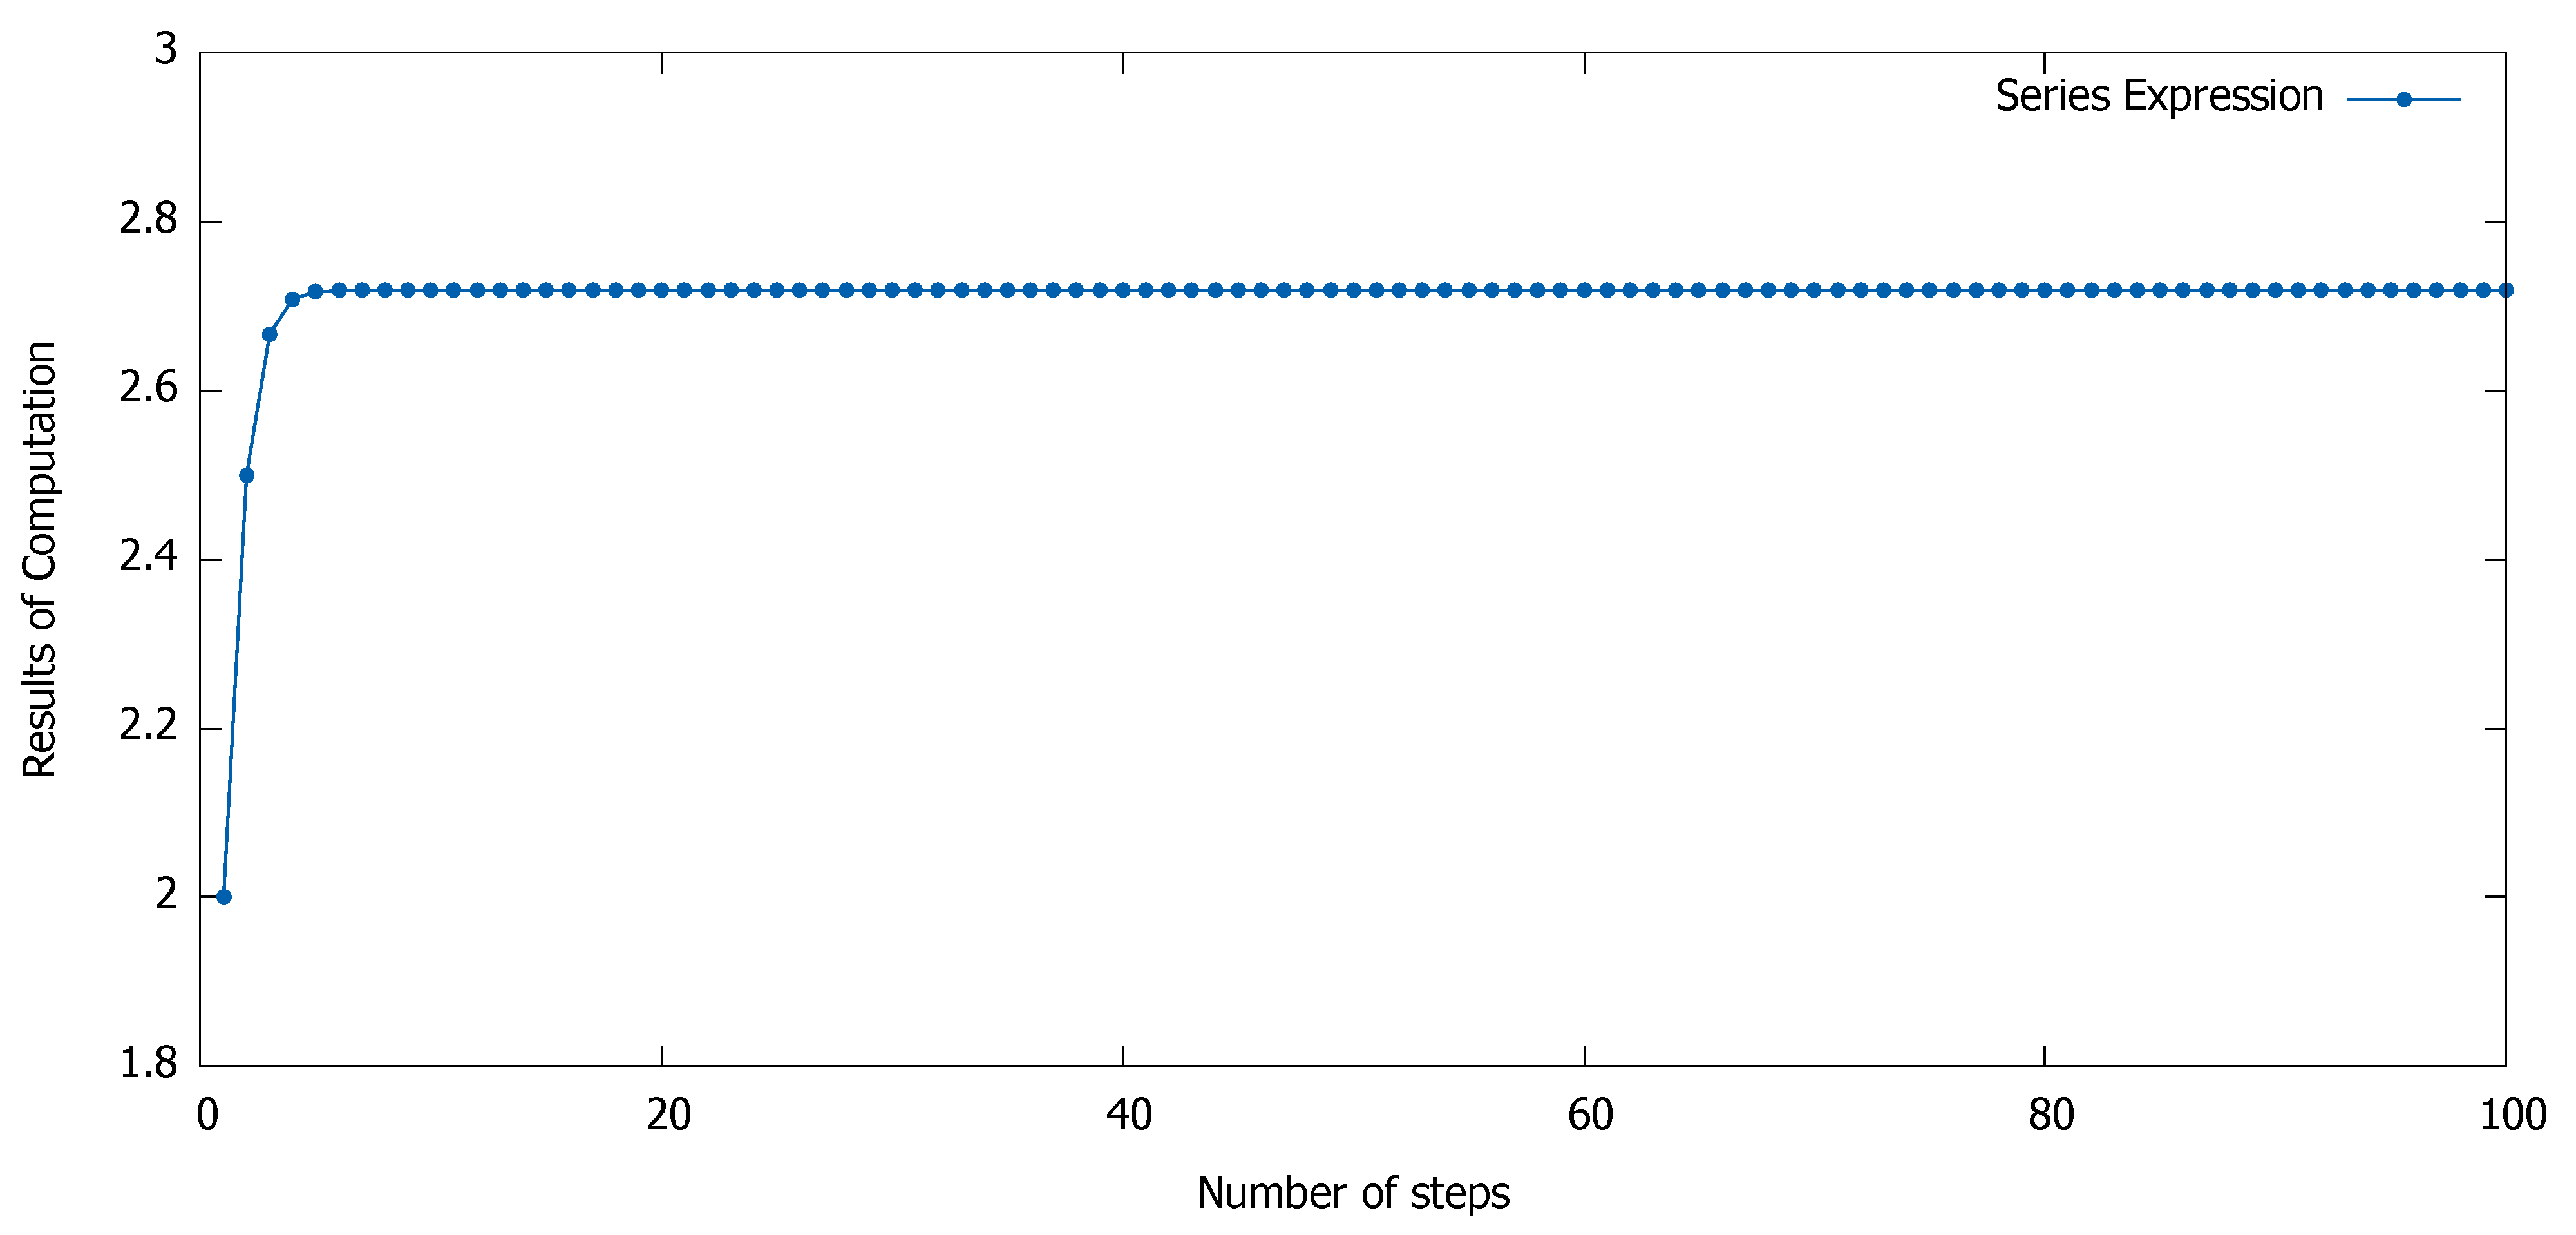
\includegraphics[scale=0.2]{data1}
   \caption{Convergence of $1+\sum_{n=1}^{\infty}\left(\frac{1}{n !}\right)$}
\end{figure} 
\begin{figure}[h]
   \centering
   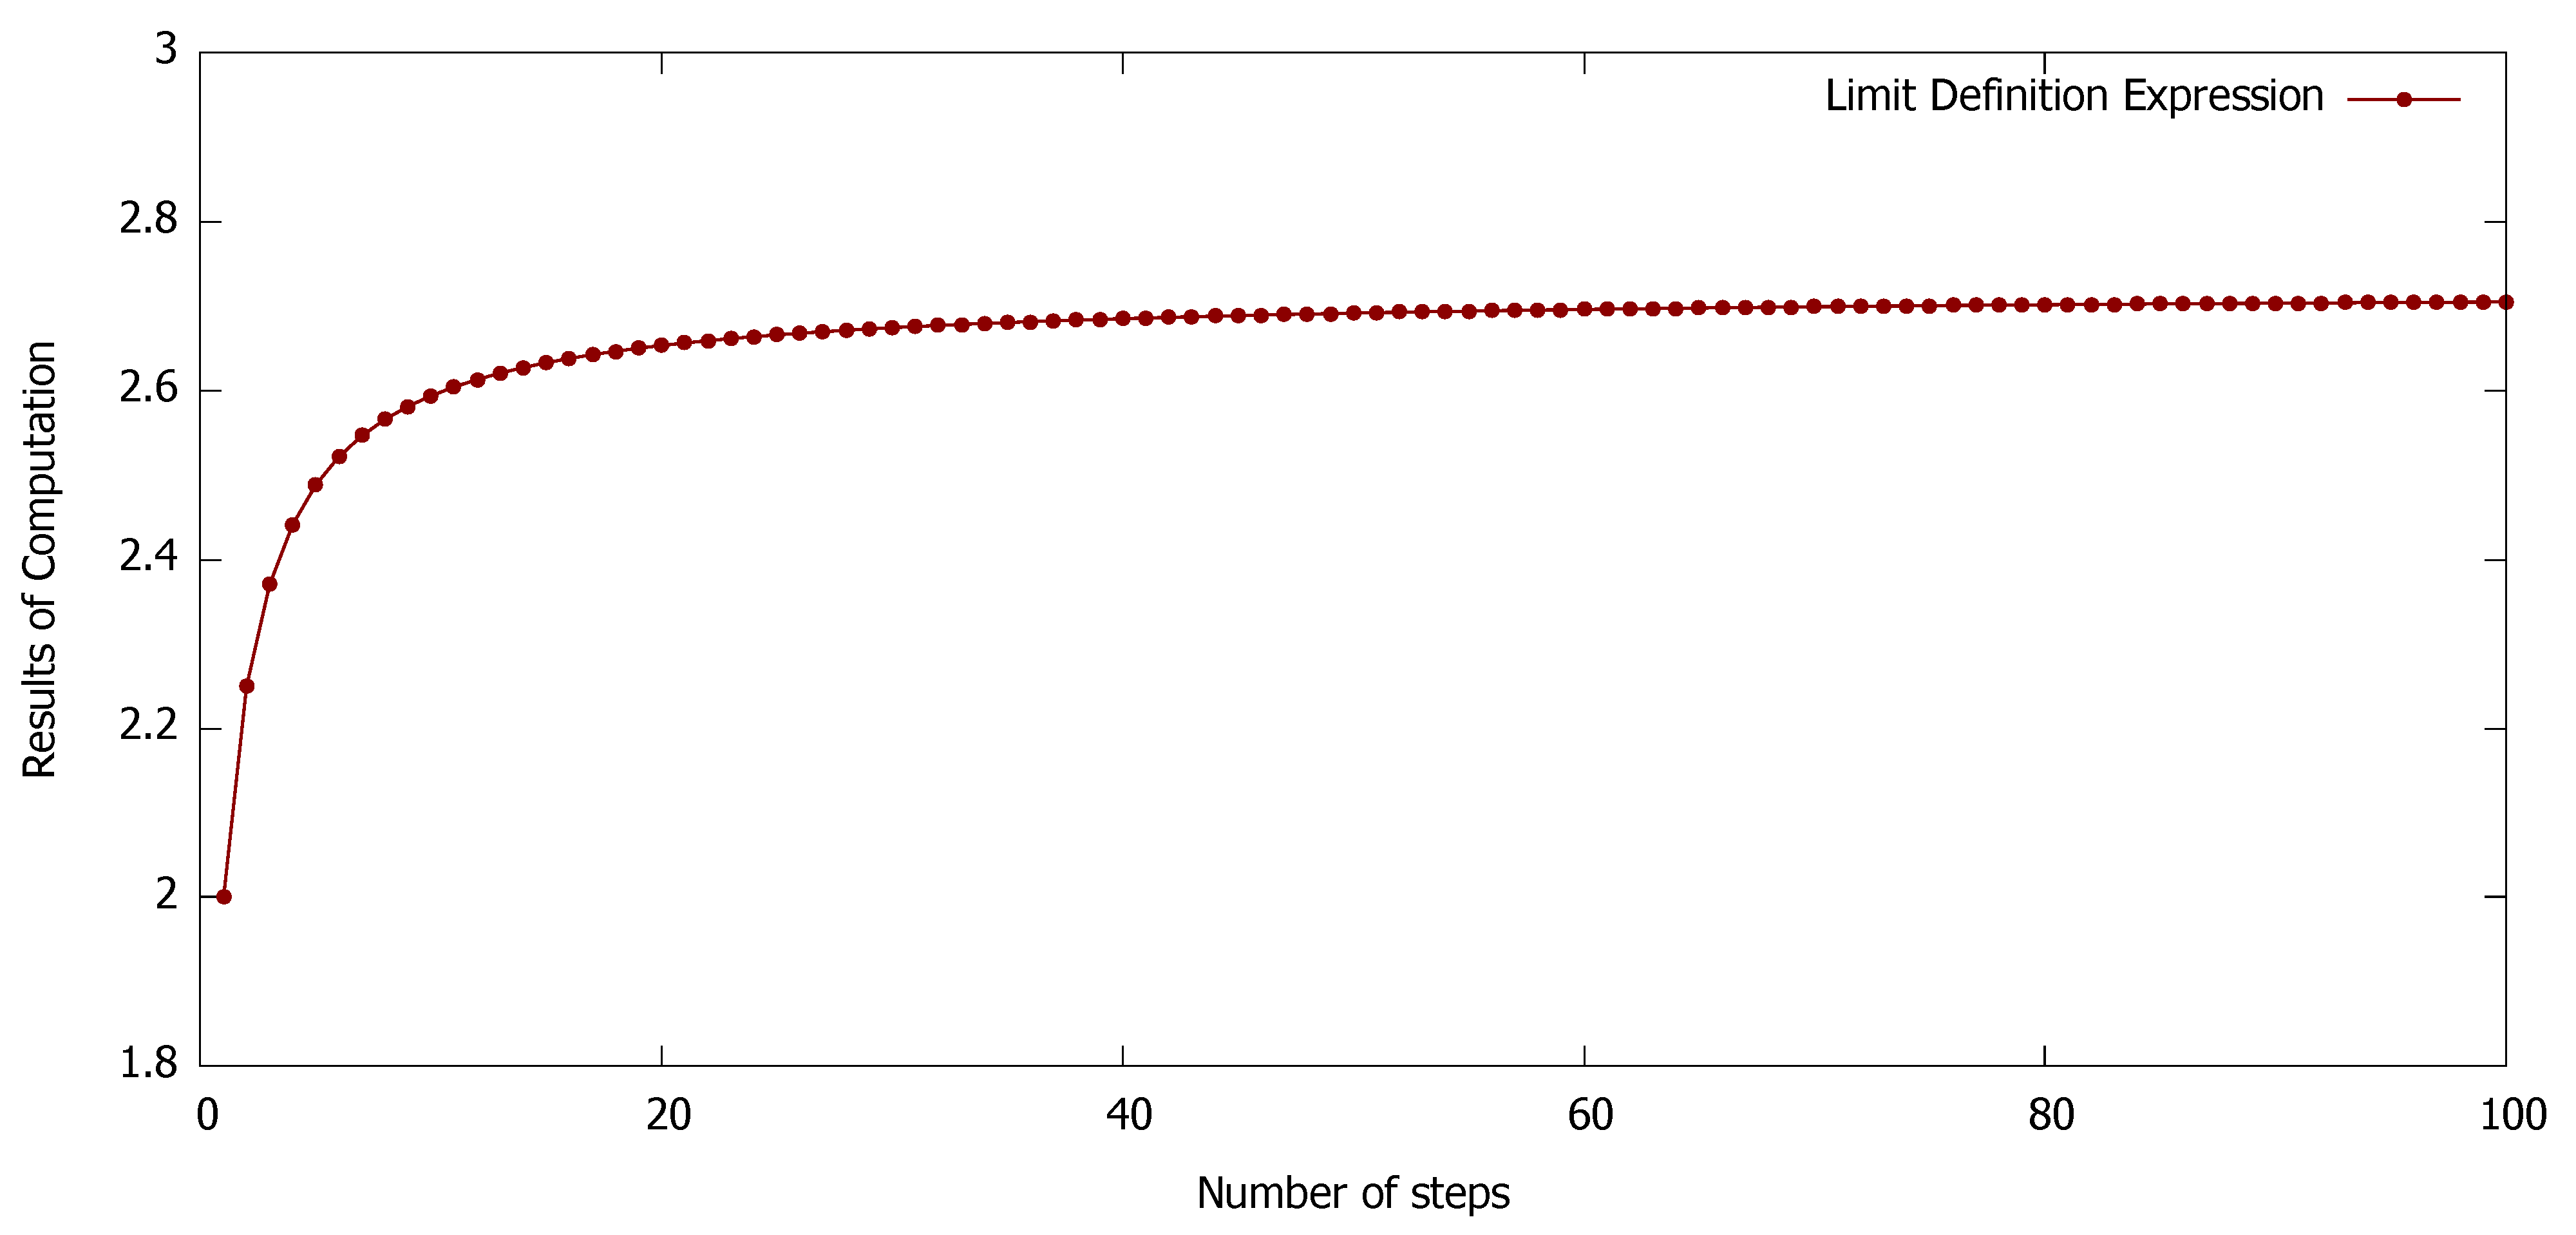
\includegraphics[scale=0.2]{data2}
   \caption{Convergence of $\lim _{n \rightarrow \infty}\left(1+\frac{1}{n}\right)^{n}$}
\end{figure} 
We could easily realize that the first expression will converge to $e$ much faster. Therefore, the first expression is much more suitable to to compute $e$.
\newpage
\section{Final Comments}
I think “Practice of Basic Informatics” is an important course that introduces the basic practice to accomplish many tasks required during the study at university. We got acquainted with the usage of Linux Operating System, Latex, Gnuplot, and FORTRAN programming language. Nevertheless, I think working with the VDI was quite inconvenient at times and it would be better to have sections that introduce other alternative environments as well as how to install the necessary tools into those.  
\end{document}